     %% bare_jrnl.tex
%% V1.4b
%% 2015/08/26
%% by Michael Shell
%% see http://www.michaelshell.org/
%% for current contact information.
%%
%% This is a skeleton file demonstrating the use of IEEEtran.cls
%% (requires IEEEtran.cls version 1.8b or later) with an IEEE
%% journal paper.
%%
%% Support sites:
%% http://www.michaelshell.org/tex/ieeetran/
%% http://www.ctan.org/pkg/ieeetran
%% and
%% http://www.ieee.org/

%%*************************************************************************
%% Legal Notice:
%% This code is offered as-is without any warranty either expressed or
%% implied; without even the implied warranty of MERCHANTABILITY or
%% FITNESS FOR A PARTICULAR PURPOSE! 
%% User assumes all risk.
%% In no event shall the IEEE or any contributor to this code be liable for
%% any damages or losses, including, but not limited to, incidental,
%% consequential, or any other damages, resulting from the use or misuse
%% of any information contained here.
%%
%% All comments are the opinions of their respective authors and are not
%% necessarily endorsed by the IEEE.
%%
%% This work is distributed under the LaTeX Project Public License (LPPL)
%% ( http://www.latex-project.org/ ) version 1.3, and may be freely used,
%% distributed and modified. A copy of the LPPL, version 1.3, is included
%% in the base LaTeX documentation of all distributions of LaTeX released
%% 2003/12/01 or later.
%% Retain all contribution notices and credits.
%% ** Modified files should be clearly indicated as such, including  **
%% ** renaming them and changing author support contact information. **
%%*************************************************************************


% *** Authors should verify (and, if needed, correct) their LaTeX system  ***
% *** with the testflow diagnostic prior to trusting their LaTeX platform ***
% *** with production work. The IEEE's font choices and paper sizes can   ***
% *** trigger bugs that do not appear when using other class files.       ***                          ***
% The testflow support page is at:
% http://www.michaelshell.org/tex/testflow/


% Please refer to your journal's instructions for other
% options that should be set.
\documentclass[journal,onecolumn]{IEEEtran}
%
% If IEEEtran.cls has not been installed into the LaTeX system files,
% manually specify the path to it like:
% \documentclass[journal]{../sty/IEEEtran}





% Some very useful LaTeX packages include:
% (uncomment the ones you want to load)


% *** MISC UTILITY PACKAGES ***
%
%\usepackage{ifpdf}
% Heiko Oberdiek's ifpdf.sty is very useful if you need conditional
% compilation based on whether the output is pdf or dvi.
% usage:
% \ifpdf
%   % pdf code
% \else
%   % dvi code
% \fi
% The latest version of ifpdf.sty can be obtained from:
% http://www.ctan.org/pkg/ifpdf
% Also, note that IEEEtran.cls V1.7 and later provides a builtin
% \ifCLASSINFOpdf conditional that works the same way.
% When switching from latex to pdflatex and vice-versa, the compiler may
% have to be run twice to clear warning/error messages.






% *** CITATION PACKAGES ***
%
%\usepackage{cite}
% cite.sty was written by Donald Arseneau
% V1.6 and later of IEEEtran pre-defines the format of the cite.sty package
% \cite{} output to follow that of the IEEE. Loading the cite package will
% result in citation numbers being automatically sorted and properly
% "compressed/ranged". e.g., [1], [9], [2], [7], [5], [6] without using
% cite.sty will become [1], [2], [5]--[7], [9] using cite.sty. cite.sty's
% \cite will automatically add leading space, if needed. Use cite.sty's
% noadjust option (cite.sty V3.8 and later) if you want to turn this off
% such as if a citation ever needs to be enclosed in parenthesis.
% cite.sty is already installed on most LaTeX systems. Be sure and use
% version 5.0 (2009-03-20) and later if using hyperref.sty.
% The latest version can be obtained at:
% http://www.ctan.org/pkg/cite
% The documentation is contained in the cite.sty file itself.






% *** GRAPHICS RELATED PACKAGES ***
%
\ifCLASSINFOpdf
\usepackage[pdftex]{graphicx}
  % declare the path(s) where your graphic files are
  % \graphicspath{{../pdf/}{../jpeg/}}
  % and their extensions so you won't have to specify these with
  % every instance of \includegraphics
  % \DeclareGraphicsExtensions{.pdf,.jpeg,.png}
\else
  % or other class option (dvipsone, dvipdf, if not using dvips). graphicx
  % will default to the driver specified in the system graphics.cfg if no
  % driver is specified.
  % \usepackage[dvips]{graphicx}
  % declare the path(s) where your graphic files are
  % \graphicspath{{../eps/}}
  % and their extensions so you won't have to specify these with
  % every instance of \includegraphics
  % \DeclareGraphicsExtensions{.eps}
\fi
% graphicx was written by David Carlisle and Sebastian Rahtz. It is
% required if you want graphics, photos, etc. graphicx.sty is already
% installed on most LaTeX systems. The latest version and documentation
% can be obtained at: 
% http://www.ctan.org/pkg/graphicx
% Another good source of documentation is "Using Imported Graphics in
% LaTeX2e" by Keith Reckdahl which can be found at:
% http://www.ctan.org/pkg/epslatex
%
% latex, and pdflatex in dvi mode, support graphics in encapsulated
% postscript (.eps) format. pdflatex in pdf mode supports graphics
% in .pdf, .jpeg, .png and .mps (metapost) formats. Users should ensure
% that all non-photo figures use a vector format (.eps, .pdf, .mps) and
% not a bitmapped formats (.jpeg, .png). The IEEE frowns on bitmapped formats
% which can result in "jaggedy"/blurry rendering of lines and letters as
% well as large increases in file sizes.
%
% You can find documentation about the pdfTeX application at:
% http://www.tug.org/applications/pdftex





% *** MATH PACKAGES ***
%
\usepackage{amsmath}
% A popular package from the American Mathematical Society that provides
% many useful and powerful commands for dealing with mathematics.
%
% Note that the amsmath package sets \interdisplaylinepenalty to 10000
% thus preventing page breaks from occurring within multiline equations. Use:
%\interdisplaylinepenalty=2500
% after loading amsmath to restore such page breaks as IEEEtran.cls normally
% does. amsmath.sty is already installed on most LaTeX systems. The latest
% version and documentation can be obtained at:
% http://www.ctan.org/pkg/amsmath





% *** SPECIALIZED LIST PACKAGES ***
%
% \usepackage{algorithmic}
% algorithmic.sty was written by Peter Williams and Rogerio Brito.
% This package provides an algorithmic environment fo describing algorithms.
% You can use the algorithmic environment in-text or within a figure
% environment to provide for a floating algorithm. Do NOT use the algorithm
% floating environment provided by algorithm.sty (by the same authors) or
% algorithm2e.sty (by Christophe Fiorio) as the IEEE does not use dedicated
% algorithm float types and packages that provide these will not provide
% correct IEEE style captions. The latest version and documentation of
% algorithmic.sty can be obtained at:
% http://www.ctan.org/pkg/algorithms
% Also of interest may be the (relatively newer and more customizable)
% algorithmicx.sty package by Szasz Janos:
% http://www.ctan.org/pkg/algorithmicx




% *** ALIGNMENT PACKAGES ***
%
%\usepackage{array}
% Frank Mittelbach's and David Carlisle's array.sty patches and improves
% the standard LaTeX2e array and tabular environments to provide better
% appearance and additional user controls. As the default LaTeX2e table
% generation code is lacking to the point of almost being broken with
% respect to the quality of the end results, all users are strongly
% advised to use an enhanced (at the very least that provided by array.sty)
% set of table tools. array.sty is already installed on most systems. The
% latest version and documentation can be obtained at:
% http://www.ctan.org/pkg/array


% IEEEtran contains the IEEEeqnarray family of commands that can be used to
% generate multiline equations as well as matrices, tables, etc., of high
% quality.


\usepackage{float}
\usepackage{graphicx}
\usepackage{hyperref}

% *** SUBFIGURE PACKAGES ***
%\ifCLASSOPTIONcompsoc
%  \usepackage[caption=false,font=normalsize,labelfont=sf,textfont=sf]{subfig}
%\else
%  \usepackage[caption=false,font=footnotesize]{subfig}
%\fi
% subfig.sty, written by Steven Douglas Cochran, is the modern replacement
% for subfigure.sty, the latter of which is no longer maintained and is
% incompatible with some LaTeX packages including fixltx2e. However,
% subfig.sty requires and automatically loads Axel Sommerfeldt's caption.sty
% which will override IEEEtran.cls' handling of captions and this will result
% in non-IEEE style figure/table captions. To prevent this problem, be sure
% and invoke subfig.sty's "caption=false" package option (available since
% subfig.sty version 1.3, 2005/06/28) as this is will preserve IEEEtran.cls
% handling of captions.
% Note that the Computer Society format requires a larger sans serif font
% than the serif footnote size font used in traditional IEEE formatting
% and thus the need to invoke different subfig.sty package options depending
% on whether compsoc mode has been enabled.
%
% The latest version and documentation of subfig.sty can be obtained at:
% http://www.ctan.org/pkg/subfig




% *** FLOAT PACKAGES ***
%
%\usepackage{fixltx2e}
% fixltx2e, the successor to the earlier fix2col.sty, was written by
% Frank Mittelbach and David Carlisle. This package corrects a few problems
% in the LaTeX2e kernel, the most notable of which is that in current
% LaTeX2e releases, the ordering of single and double column floats is not
% guaranteed to be preserved. Thus, an unpatched LaTeX2e can allow a
% single column figure to be placed prior to an earlier double column
% figure.
% Be aware that LaTeX2e kernels dated 2015 and later have fixltx2e.sty's
% corrections already built into the system in which case a warning will
% be issued if an attempt is made to load fixltx2e.sty as it is no longer
% needed.
% The latest version and documentation can be found at:
% http://www.ctan.org/pkg/fixltx2e


%\usepackage{stfloats}
% stfloats.sty was written by Sigitas Tolusis. This package gives LaTeX2e
% the ability to do double column floats at the bottom of the page as well
% as the top. (e.g., "\begin{figure*}[!b]" is not normally possible in
% LaTeX2e). It also provides a command:
%\fnbelowfloat
% to enable the placement of footnotes below bottom floats (the standard
% LaTeX2e kernel puts them above bottom floats). This is an invasive package
% which rewrites many portions of the LaTeX2e float routines. It may not work
% with other packages that modify the LaTeX2e float routines. The latest
% version and documentation can be obtained at:
% http://www.ctan.org/pkg/stfloats
% Do not use the stfloats baselinefloat ability as the IEEE does not allow
% \baselineskip to stretch. Authors submitting work to the IEEE should note
% that the IEEE rarely uses double column equations and that authors should try
% to avoid such use. Do not be tempted to use the cuted.sty or midfloat.sty
% packages (also by Sigitas Tolusis) as the IEEE does not format its papers in
% such ways.
% Do not attempt to use stfloats with fixltx2e as they are incompatible.
% Instead, use Morten Hogholm'a dblfloatfix which combines the features
% of both fixltx2e and stfloats:
%
% \usepackage{dblfloatfix}
% The latest version can be found at:
% http://www.ctan.org/pkg/dblfloatfix




%\ifCLASSOPTIONcaptionsoff
%  \usepackage[nomarkers]{endfloat}
% \let\MYoriglatexcaption\caption
% \renewcommand{\caption}[2][\relax]{\MYoriglatexcaption[#2]{#2}}
%\fi
% endfloat.sty was written by James Darrell McCauley, Jeff Goldberg and 
% Axel Sommerfeldt. This package may be useful when used in conjunction with 
% IEEEtran.cls'  captionsoff option. Some IEEE journals/societies require that
% submissions have lists of figures/tables at the end of the paper and that
% figures/tables without any captions are placed on a page by themselves at
% the end of the document. If needed, the draftcls IEEEtran class option or
% \CLASSINPUTbaselinestretch interface can be used to increase the line
% spacing as well. Be sure and use the nomarkers option of endfloat to
% prevent endfloat from "marking" where the figures would have been placed
% in the text. The two hack lines of code above are a slight modification of
% that suggested by in the endfloat docs (section 8.4.1) to ensure that
% the full captions always appear in the list of figures/tables - even if
% the user used the short optional argument of \caption[]{}.
% IEEE papers do not typically make use of \caption[]'s optional argument,
% so this should not be an issue. A similar trick can be used to disable
% captions of packages such as subfig.sty that lack options to turn off
% the subcaptions:
% For subfig.sty:
% \let\MYorigsubfloat\subfloat
% \renewcommand{\subfloat}[2][\relax]{\MYorigsubfloat[]{#2}}
% However, the above trick will not work if both optional arguments of
% the \subfloat command are used. Furthermore, there needs to be a
% description of each subfigure *somewhere* and endfloat does not add
% subfigure captions to its list of figures. Thus, the best approach is to
% avoid the use of subfigure captions (many IEEE journals avoid them anyway)
% and instead reference/explain all the subfigures within the main caption.
% The latest version of endfloat.sty and its documentation can obtained at:
% http://www.ctan.org/pkg/endfloat
%
% The IEEEtran \ifCLASSOPTIONcaptionsoff conditional can also be used
% later in the document, say, to conditionally put the References on a 
% page by themselves.

\usepackage{subfigure}



% *** PDF, URL AND HYPERLINK PACKAGES ***
%
%\usepackage{url}
% url.sty was written by Donald Arseneau. It provides better support for
% handling and breaking URLs. url.sty is already installed on most LaTeX
% systems. The latest version and documentation can be obtained at:
% http://www.ctan.org/pkg/url
% Basically, \url{my_url_here}.




% *** Do not adjust lengths that control margins, column widths, etc. ***
% *** Do not use packages that alter fonts (such as pslatex).         ***
% There should be no need to do such things with IEEEtran.cls V1.6 and later.
% (Unless specifically asked to do so by the journal or conference you plan
% to submit to, of course. )


% correct bad hyphenation here
\hyphenation{op-tical net-works semi-conduc-tor}

\usepackage{mathtools}
\begin{document}
%
% paper title
% Titles are generally capitalized except for words such as a, an, and, as,
% at, but, by, for, in, nor, of, on, or, the, to and up, which are usually
% not capitalized unless they are the first or last word of the title.
% Linebreaks \\ can be used within to get better formatting as desired.
% Do not put math or special symbols in the title.
\title{High-order Finite Volume Methods}
%
%
% author names and IEEE memberships
% note positions of commas and nonbreaking spaces ( ~ ) LaTeX will not break
% a structure at a ~ so this keeps an author's name from being broken across
% two lines.
% use \thanks{} to gain access to the first footnote area
% a separate \thanks must be used for each paragraph as LaTeX2e's \thanks
% was not built to handle multiple paragraphs
%

\author{Oguz~Ziya~Koseomur,~\IEEEmembership{Computational Science and Engineering, Technical University Munich}}

% note the % following the last \IEEEmembership and also \thanks - 
% these prevent an unwanted space from occurring between the last author name
% and the end of the author line. i.e., if you had this:
% 
% \author{....lastname \thanks{...} \thanks{...} }
%                     ^------------^------------^----Do not want these spaces!
%
% a space would be appended to the last name and could cause every name on that
% line to be shifted left slightly. This is one of those "LaTeX things". For
% instance, "\textbf{A} \textbf{B}" will typeset as "A B" not "AB". To get
% "AB" then you have to do: "\textbf{A}\textbf{B}"
% \thanks is no different in this regard, so shield the last } of each \thanks
% that ends a line with a % and do not let a space in before the next \thanks.
% Spaces after \IEEEmembership other than the last one are OK (and needed) as
% you are supposed to have spaces between the names. For what it is worth,
% this is a minor point as most people would not even notice if the said evil
% space somehow managed to creep in.



% The paper headers
\markboth{Fundamentals of Wave Simulation - Solving Hyperbolic Systems of PDEs, Winter 2020/2021}%
{Shell \MakeLowercase{\textit{et al.}}: Bare Demo of IEEEtran.cls for IEEE Journals}
% The only time the second header will appear is for the odd numbered pages
% after the title page when using the twoside option.
% 
% *** Note that you probably will NOT want to include the author's ***
% *** name in the headers of peer review papers.                   ***
% You can use \ifCLASSOPTIONpeerreview for conditional compilation here if
% you desire.




% If you want to put a publisher's ID mark on the page you can do it like
% this:
%\IEEEpubid{0000--0000/00\$00.00~\copyright~2015 IEEE}
% Remember, if you use this you must call \IEEEpubidadjcol in the second
% column for its text to clear the IEEEpubid mark.



% use for special paper notices
%\IEEEspecialpapernotice{(Invited Paper)}




% make the title area
\maketitle

% As a general rule, do not put math, special symbols or citations
% in the abstract or keywords.
\begin{abstract}
 In this review, the main ingredients of high-order finite volume methods are reviewed. First, Godunov's method for the linear systems, the \textit{Reconstruct-Evolve-Average (REA)} algorithm is introduced. This algorithm is the basis for the development of most high order methods and it is mainly based on the polynomial reconstruction of the data. Then, the monotonic upstream-centered scheme for conservation laws (MUSCL) as well as the total variation and the total variation diminishing (TVD) methods are discussed, which are aimed to bound the oscillations in the solution. A method to obtain higher resolution in the temporal domain, the semi-discrete form, is introduced. Semi-discrete form allows us to decouple issues of the temporal discretization and the spatial discretization. Finally, more advanced methods to reconstruct the higher order polynomials, such as Newton's divided differences, essentially non-oscillatory schemes are briefly mentioned. Most of the discussions and derivations are centered around the linear equations.
\end{abstract}

% Note that keywords are not normally used for peerreview papers.
\begin{IEEEkeywords}
finite volumes, high-order, limiters, TVD, total variation, MUSCL, ENO, WENO
\end{IEEEkeywords}






% For peer review papers, you can put extra information on the cover
% page as needed:
% \ifCLASSOPTIONpeerreview
% \begin{center} \bfseries EDICS Category: 3-BBND \end{center}
% \fi
%
% For peerreview papers, this IEEEtran command inserts a page break and
% creates the second title. It will be ignored for other modes.
\IEEEpeerreviewmaketitle

\section{Introduction}
% The very first letter is a 2 line initial drop letter followed
% by the rest of the first word in caps.
% 
% form to use if the first word consists of a single letter:
% \IEEEPARstart{A}{demo} file is ....
% 
% form to use if you need the single drop letter followed by
% normal text (unknown if ever used by the IEEE):
% \IEEEPARstart{A}{}demo file is ....
% 
% Some journals put the first two words in caps:
% \IEEEPARstart{T}{his demo} file is ....
% 
% Here we have the typical use of a "T" for an initial drop letter
% and "HIS" in caps to complete the first word.
\IEEEPARstart{T}{he} upwind method for hyperbolic PDEs showed great success overcoming the instabilities introduced with central schemes. However, a trade-off for the accuracy has been made to make the solutions more stable. In addition, this method is highly dissipative, therefore it tends to smooth the solution, which is not accurate for the discontinuous solutions. These discontinuities can either be introduced as initial conditions or the artifacts of the non-linear equations. Considering this, we expect a numerical method to behave well in smooth regions as well as in discontinuous regions. Since the finite volume methods consists of several steps, it is not trivial to introduce the stable higher order methods, unlike finite differences. A special care must be taken in each step of the development of the solution, such as representing the data as a continuous set of points, while not smoothing the data in the discontinuous regions, accomplishing integration and differentiation operations in both spatial and temporal domains without loss of accuracy. In addition, we should also consider their effects on each other too. As a result, a systematic, reproducible procedure with a mathematical background is necessary to develop the high-order methods.
\par
Most of the methods are tested and compared using the linear advection equation with constant velocity. The advection velocity, $\Bar{u}$, is assumed to be positive and constant in order to reduce the complexity in the derivations.
\begin{equation} \label{advection}
    q_t + \Bar{u}q_x = 0
\end{equation}
\par
In the following sections, first, the main algorithm for the most of the methods, \textit{reconstruct-evolve-average} algorithm and a second order method and its drawbacks, the Lax-Wendroff method are introduced. Then, the methods to blend high order methods with the lower order methods without adding oscillations to our solutions, the limiters and MUSCL method, are discussed. Methods for the temporal high resolution are introduced and the paper is finalized with the more advanced methods for the polynomial reconstruction, ENO and WENO methods.

\section{Reconstruct-Evolve-Average (REA) Algorithm}
REA algorithm is the upwind method for systems of equations and plays an important role to develop high-order methods. The method consists of three main steps:
\begin{enumerate}
    \item \textbf{Reconstruct:} On the discretized domain, construct a piecewise polynomial using the cell averages. Denoting $P$ as the piecewise polynomial constructed from cell averages, $Q_i^{n}$, 
    
    $$
        \tilde{q}^{n}(x, t_{n}) = P(x)
    $$
    
    \item \textbf{Evolve:} In this step, time marching for one time step is performed for the reconstructed state. 
    
    $$
        \tilde{q}^{n}(x, t_{n}) \longrightarrow \tilde{q}^{n}(x, t_{n+1})
    $$
    
    \item \textbf{Average:} Reconstruction of the cell values requires the average values for each cell on cell centers. Therefore, the evolved state is averaged over each cell, in a conservative fashion. 
    
    $$
        Q_i^{n+1} = \frac{1}{\Delta x}\int_{C_i}  \tilde{q}^{n}(x, t_{n+1}) dx
    $$
    
    Then the algorithm repeats itself.
\end{enumerate}

The simplest choice for the reconstruction in the step 1 is using a piecewise constant polynomial to represent the data, which is also the original version of the algorithm. This construction leads to the basic Riemann problems. However, this approach only results in first order accuracy. In order to obtain better accuracy, one should use better reconstruction approaches, which are discussed in the next sections. The finite volume realization of this algorithm with the numerical flux can be derived as follows in Equations \ref{god1} to \ref{god3}. Recalling the numerical flux definition:
$$
    F_{i-1/2}^n \approx \frac{1}{\Delta x} \int_{t_n}^{t_{n+1}} f(q(x_{i-1}, t))dt
$$
\newline
which approximates the flux between the cells $i-1$ and $i$. Instead of using the exact value $q(x, t)$ in the integral, piecewise version $\tilde{q}(x, t)$ can be used, in which the calculation of the respective integral is exact. Then the algorithm reduces to:

\begin{enumerate}
    \item Solve the Riemann problem on the interface $x_{i-1/2}$
    \begin{equation} \label{god1}
        Q^*_{i-1/2} = R(Q_{i-1}, Q_{i})
    \end{equation}
    where the $R$ represents an exact or approximate Riemann solver and the $Q^*_{i-1/2}$ represents the solution of the Riemann problem.
    
    \item Calculate the flux as
     \begin{equation} \label{god2}
        {F}_{i-1/2} = F(Q_{i-1}, Q_i) = f(Q^*_{i-1/2})
     \end{equation}
    \item Apply flux-differencing formula to obtain the next state
    
    \begin{equation} \label{god3}
         Q_i^{n+1} = Q_i^{n} - \frac{\Delta t}{\Delta x}({F}_{i+1/2} - {F}_{i-1/2})
    \end{equation}
    
\end{enumerate}

Consider the linear advection equation given in the Eq. \ref{advection}. With the first order upwind method, Equation \ref{god3} reduces to:
$$
    Q_i^{n+1} = Q_i^{n} - \frac{\Bar{u}\Delta t}{\Delta x}({Q}^n_{i} - {Q}^n_{i-1})
$$
which is the update formula for the first-order upwind method of Godunov, and the most common presentation of the REA algorithm.

\section{Lax-Wendroff Method}
The Lax-Wendroff method is a second order method which is derived from the Taylor series expansion. For the linear advection equation in Eq. \ref{advection}, differentiation of this equation with respect to $t$ gives
$$
q_{tt} = - \Bar{u} q_{xt} = -\Bar{u}(-\Bar{u} q_x)_x = \Bar{u}^2 q_{xx}
$$
since the $q_{xt} = q_{tx}$. As for the next step, we can use the Taylor series expansion in the temporal domain to expand the next time step
$$
q(x, t_{n+1}) = q(x, t_n) + \Delta t q_t(x, t_n) + \frac{1}{2}(\Delta t)^2 q_{tt}(x, t_n) + O(\Delta t^3)
$$
Now, we can replace the derivatives with respect to $t$ to $x$ using the previous relation as
$$
q(x, t_{n+1}) = q(x, t_n) - \Bar{u} \Delta t q_x(x, t_n) + \frac{1}{2}(\Delta t)^2 \Bar{u}^2 q_{xx}(x, t_n) + O(\Delta t^3)
$$
Finally, keeping only up to the third order error term and replacing the differentials with the central differences and exact values with the cell averages, we obtain the update formula of the Lax-Wendroff method. 
$$
    Q_i^{n+1} = Q_i^{n} - \frac{\Bar{u} \Delta t}{2\Delta x}(Q^n_{i+1}-Q^n_{i-1}) + \frac{1}{2}\left(\frac{\Bar{u}\Delta t}{\Delta x}\right)^2 (Q^n_{i+1} - 2Q^n_{i} +  Q^n_{i-1})
$$

The Lax-Wendroff method is a second order method as opposed to the first order upwind method. However, in case of a discontinuity in the solution, it begins to produce unphysical oscillations. This is mainly due to the dispersive nature of the error term, third derivative. In addition, this dispersive error also causes some kind of phase shift even in the smooth regions. For example, Figure \ref{fig:lax_wendroff} compares the first order-upwind method and the Lax-Wendroff method on advection equation. While the first order upwind method results in dissipative results, the Lax-Wendroff method shows highly oscillatory behaviour.

\begin{figure}
    \centering
    \begin{subfigure}{\textwidth}
    \centering
    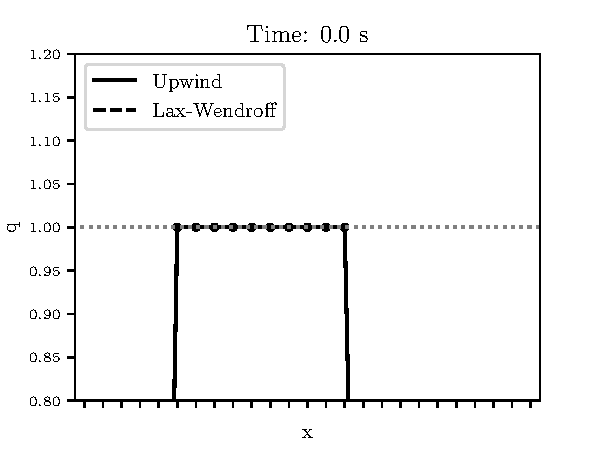
\includegraphics[width=0.3\textwidth]{figures/lax-initial.pdf}
    \end{subfigure}
    \begin{subfigure}{\textwidth}
    \centering
    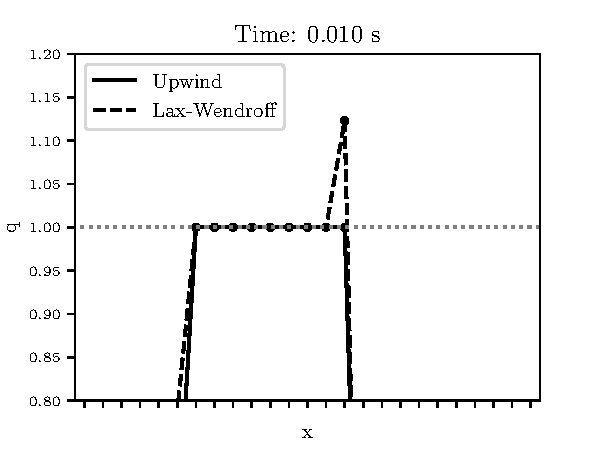
\includegraphics[width=0.3\textwidth]{figures/lax0.010.pdf}
    \end{subfigure}
    \begin{subfigure}{\textwidth}
    \centering
    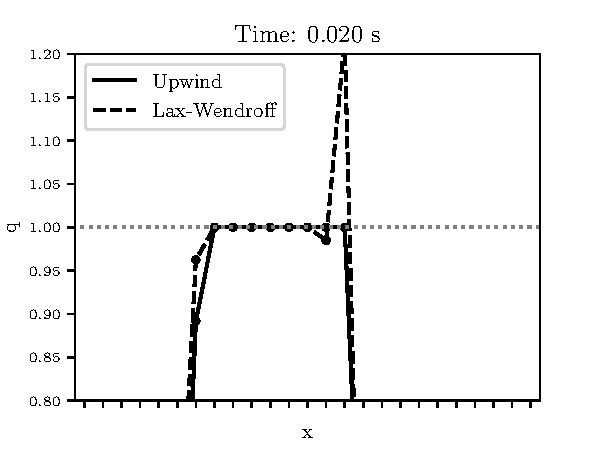
\includegraphics[width=0.3\textwidth]{figures/lax0.020.pdf}
    \end{subfigure}
    \begin{subfigure}{\textwidth}
    \centering
    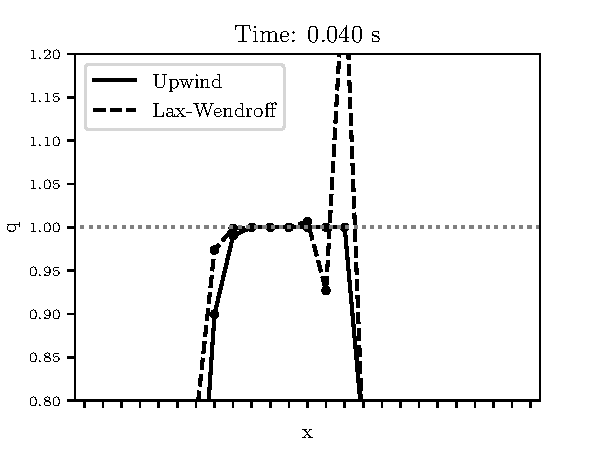
\includegraphics[width=0.3\textwidth]{figures/lax0.040.pdf}
    \end{subfigure}
    \begin{subfigure}{\textwidth}
    \centering
    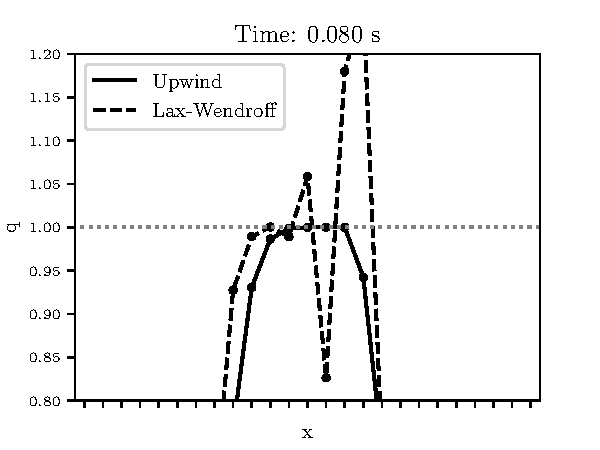
\includegraphics[width=0.3\textwidth]{figures/lax0.080.pdf}
    \end{subfigure}
        \begin{subfigure}{\textwidth}
    \centering
    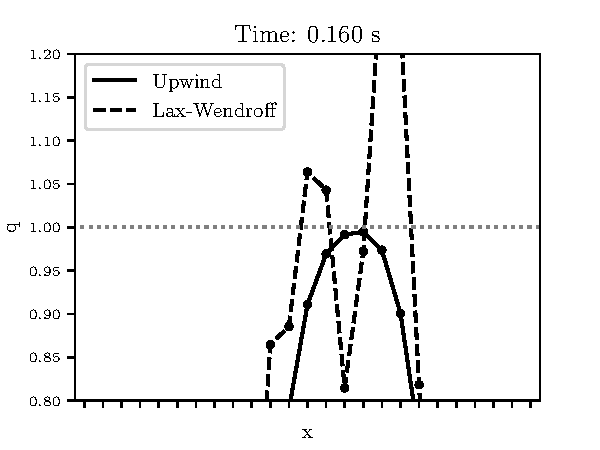
\includegraphics[width=0.3\textwidth]{figures/lax0.160.pdf}
    \end{subfigure}
    \caption{Evolution of the step initial condition under the advection equation with the first order upwind and Lax-Wendroff methods. CFL number is 0.3. The highly oscillatory behaviour of the Lax-Wendroff method is clearly visible from the first time step.}
    \label{fig:lax_wendroff}
\end{figure}

\newline
To summarize, we get a highly dissipative, low order but non-oscillatory solution with upwind method, while we get a high order but oscillatory solution near discontinuities. The idea of limiting tries to combine the best features of both methods: high order solution in the smooth regions, non-oscillatory solution near discontinuities. Keeping this in mind, the Lax-Wendroff method is an important method to characterize higher order methods developed later in this paper.

\section{Reconstruction}
In the REA algorithm, cell averages are reconstructed using the piecewise constant polynomial. However, it appears that this reconstruction is one of the limiting cases to obtain high order methods. Instead of the piecewise constant reconstruction, a better, and simple reconstruction is linear piecewise reconstruction, such that:
$$
    \tilde{q}^n(x, t_n) = Q^n_i + \sigma_i^n(x - x_i)
$$
Two main properties of this reconstruction are the value at the cell center is equal to $Q_i^n$. In addition, the integral over the cell is equal to $Q_n^i$, no matter what the slope $\sigma_i^n$ is and this is crucial to obtain conservative schemes.
\par
After a straightforward but long derivation with the piecewise linear reconstruction, one can obtain the following general form:
\begin{equation}
        Q_i^{n+1} = Q_i^{n} - \frac{\Bar{u}\Delta t}{\Delta x}({Q}^n_{i} - {Q}^n_{i-1}) - \frac{1}{2}\frac{\Bar{u}\Delta t}{\Delta x}(\Delta x - \Bar{u}\Delta t)(\sigma_i^n - \sigma^n_{i-1})
\end{equation}

It is simply the first order upwind method with correction which depends on the slopes.

\subsection{How to Choose Slopes?}
Currently, the slopes are the free parameters for the Equation 2. As in derivative approximation, 
one can choose the following slopes without loss of generality
\newline
\begin{center}
\begin{tabular}{c|c|c}
     Centered Slope (CS) & Upwind Slope (US) & Downwind Slope (DS) \\
     \hline 
     $\sigma_i^n = (Q^n_{i+1} - Q^n_{i-1})/(2\Delta x)$ & $\sigma_i^n = (Q^n_{i} - Q^n_{i-1})/(\Delta x)$ & $\sigma_i^n = (Q^n_{i+1} - Q^n_{i})/(\Delta x)$
\end{tabular}
\end{center}
\newline

The main downside of these slopes is that they are derived such that the solution is smooth. Despite their simplicity, this assumption is invalid near discontinuities and they tend to overshoot the values depending on their direction bias, which grow over the time and create oscillatory solutions. Therefore, we need to focus on the slopes which do not add additional oscillations.

\subsection{Total Variation}
In the previous section, the overshooting behaviour of the trivial slope choices are mentioned. In order to choose more sophisticated slopes which do not have oscillatory behaviour, a function that measures oscillations should be derived. This function is denoted as Total Variation (TV) and defined as:

$$
    TV(Q) = \sum_{-\infty}^{\infty} | Q_i - Q_{i-1} |
$$

This function basically represents how oscillatory the solution is. For example, the linear advection equation with constant velocity cannot introduce additional oscillations in its nature, so the total variation of the linear advection equation is expected to be constant over time. Therefore, the numerical method used to solve this problem should not introduce additional oscillations too. Based on this, a numerical method is called total variation diminishing (TVD) if
$$
    TV(Q^n) \geq TV(Q^{n+1})
$$
This property is extremely important for a method to have non-oscillatory characteristic.

\subsection{MUSCL-Type Schemes}
Monotone Upstream-Centered Scheme for Conservation Laws, MUSCL, type schemes are the the general category of the methods in which the degree of the reconstructed polynomial is higher than the zero, which means non-constant reconstruction. Another property of the MUSCL schemes is that the higher order reconstruction should not introduce additional oscillations, as mentioned in the trivial slope selections.
\par
When the reconstruction is not constant, the definition of the Riemann problem is violated. Therefore, the Generalized Riemann Problem is defined such that the values at the cell centers are considered to compute the in-cell fluxes for the problem
$$
q_t + f(q) = 0
$$
\[ q(x,0) =   \left\{
\begin{array}{ll}
      q_i^R(x), & x < 0 \\
      q_{i+1}^L(x), & x > 0
\end{array} 
\right. \]
Moreover, the MUSCL-type schemes are not only limited with the linear reconstruction, also the higher-order reconstructions are possible. 
\par
A specific type of the MUSCL-type method, the MUSCL-Hancock method follows the algorithmic procedure given in equations \ref{muscl1} to \ref{muscl5}.

\begin{enumerate}
    \item Reconstruct the data with the linear reconstruction:
    \begin{equation}\label{muscl1}
         Q^L_i = Q_i^n - \frac{1}{2}\Delta x
    \end{equation}
    \begin{equation} \label{muscl2}
        Q^R_i = Q_i^n + \frac{1}{2}\Delta x
    \end{equation} 
    \item Evolve the solution by a time $0.5\Delta t$
    \begin{equation} \label{muscl3}
        \Bar{Q}^L_i = Q^L_i + \frac{1}{2}\frac{\Delta t}{\Delta x}(F_{i-1/2} - F_{i+1/2})
    \end{equation} \label{muscl4}
    \begin{equation}
         \Bar{Q}^R_i = Q^R_i + \frac{1}{2}\frac{\Delta t}{\Delta x}(F_{i-1/2} - F_{i+1/2})
    \end{equation}
       
    \item Solve the Generalized Riemann problem on the interface with the piecewise constant data
    \begin{equation} \label{muscl5}
    q(x,0) =  \left\{
        \begin{array}{ll}
            Q_i^R(x), & x < 0 \\
            Q_{i+1}^L(x), & x > 0
        \end{array} \right\}
    \end{equation} 
\end{enumerate}

\subsection{TVD Limiters}
Considering TVD property, more sophisticated slopes can be derived, such as
\begin{center}
\begin{tabular}{c|c|c}
     MinMod & SuperBee & MC \\
     \hline 
     $minmod (US, DS)$ & $maxmod [ minmod (DS, 2US), minmod (2DS, US) ]$ & $minmod (CS, 2US, 2DS)$
\end{tabular}
\end{center}
\newline

The MinMod slope calculates the both upwind and downwind slopes and chooses the smaller one to introduce less oscillations. If the signs are different for these slopes, then it decides on the slope of zero. This results in sharper reconstruction of the discontinuity without introducing additional oscillations. Similarly, the SuperBee slope also computes different sided slopes, but it chooses the one with the larger modulus. Monotonized central-difference limiter (MC) is one of the default choices for the most of the problems, since it chooses the central scheme when the solution is smooth therefore it does not introduce artificial effects on the smooth regions.
\par
Although the formulation for the slope-limiting is trivial and intuitive, it is not in the flux-formulation yet. Beginning from the slope-limiting, the general formulation for the flux-limited numerical methods can be derived. In this way, we can obtain the flux-limiter counterparts of the slope-limiters. The key point is that now, we associate the slope with the interface rather than the each cell. Defining the jump between the cells $i$ and $i-1$:
$$
    \Delta Q^n_{i-1/2} = Q^n_i - Q_{i-1}^n 
$$
Then the limited version of the flux on this face can be written as (given that $\Bar{u} > 0$):
$$
    F_{i-1/2}^n = \Bar{u}Q_i^n + \frac{1}{2}\Bar{u}\left(1 - \frac{\Bar{u\Delta t}}{\Delta x}\right) \phi(\theta^n_{i-1/2})\Delta Q^n_{i-1/2}
$$
where the $\phi$ is the limiter function while the $\theta$ determines the smoothness and is defined as:
$$
    \theta_{i-1/2}^n = \frac{\Delta Q^n_{i-3/2}}{\Delta Q^n_{i-1/2}}
$$
The flux-limiters defined in the previous section can be extended in this notation for the linear methods (left) and the non-linear methods (right) as:

\begin{center}
\begin{subtable}{\textwidth}
    \begin{tabular}{c|c}
         Upwind & $\phi(\theta) = 0$ \\
         \\
         \hline
         \\
         Lax-Wendroff & $\phi(\theta) = 1$ \\
         \\
         \hline
         \\
         Beam-Warming & $\phi(\theta) = \theta$ \\
         \\
         \hline
         \\
         Fromm & $\phi(\theta) = 0.5(1+\theta)$
    \end{tabular}
\end{subtable}
\begin{subtable}{\textwidth}
    \begin{tabular}{c|c}
     MinMod & $\phi(\theta) = minmod(1, \theta)$ 
     \\ \\
     \hline
     \\
     SuperBee & $\phi(\theta) = max(0, min(1, 2\theta), min(2, \theta))$ 
     \\ \\
     \hline
     \\
     MC & $\phi(\theta) = max(0, min((1 + \theta)/2, 2, \theta)$
     \\ \\
     \hline
     \\
     van Leer & $\phi(\theta) = 0.5(1+\theta)$
\end{tabular}

\end{subtable}
\end{center}

If we apply these limiters to the advection equation which was discussed in Figure \ref{fig:lax_wendroff}, it can be seen that the limiters help to capture the discontinuity sharper.

\begin{figure}
    \centering
    \begin{subfigure}{\textwidth}
    \centering
    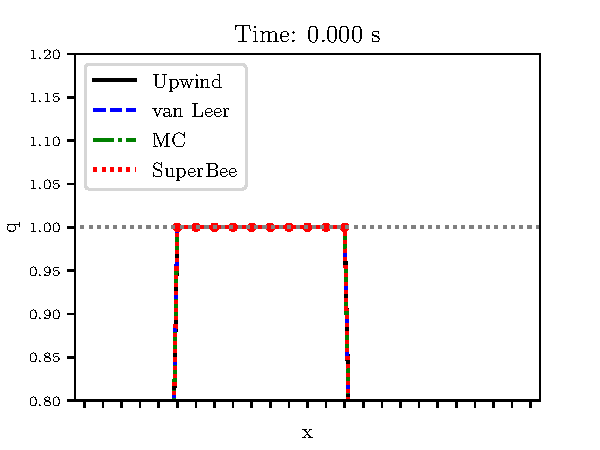
\includegraphics[width=0.3\textwidth]{figures/limiter_initial.pdf}
    \end{subfigure}
    \begin{subfigure}{\textwidth}
    \centering
    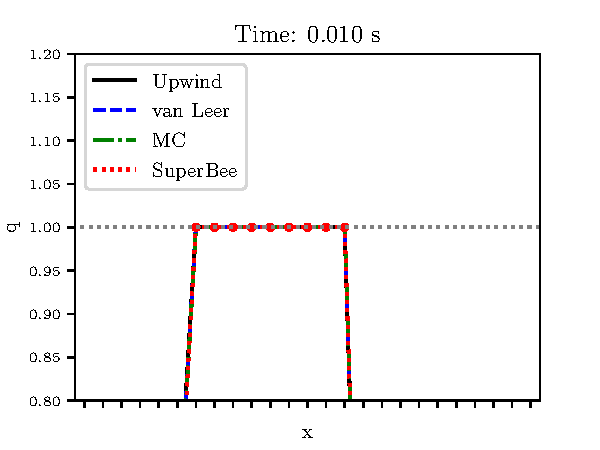
\includegraphics[width=0.3\textwidth]{figures/limiter0.010.pdf}
    \end{subfigure}
    \begin{subfigure}{\textwidth}
    \centering
    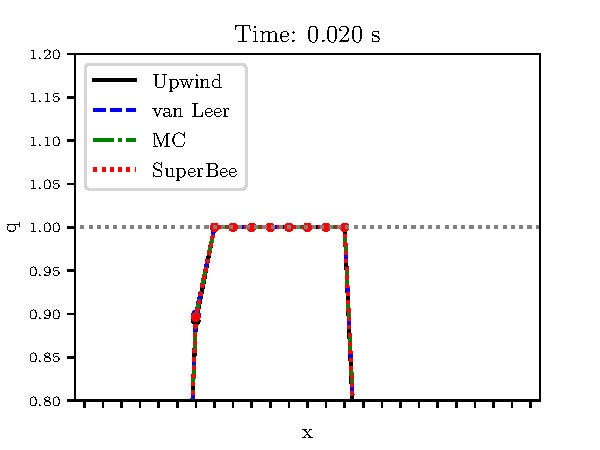
\includegraphics[width=0.3\textwidth]{figures/limiter0.020.pdf}
    \end{subfigure}
    \begin{subfigure}{\textwidth}
    \centering
    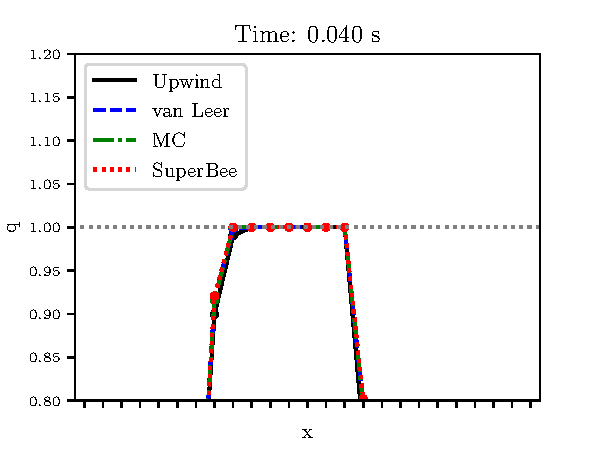
\includegraphics[width=0.3\textwidth]{figures/limiter0.040.pdf}
    \end{subfigure}
    \begin{subfigure}{\textwidth}
    \centering
    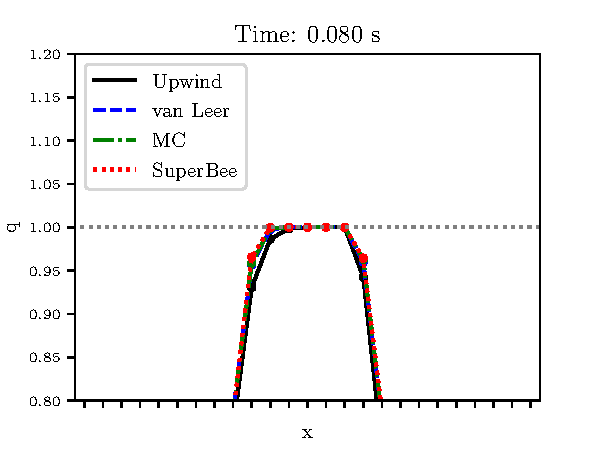
\includegraphics[width=0.3\textwidth]{figures/limiter0.080.pdf}
    \end{subfigure}
        \begin{subfigure}{\textwidth}
    \centering
    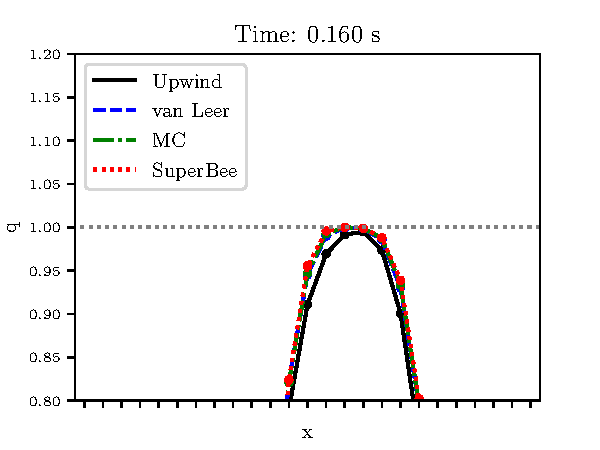
\includegraphics[width=0.3\textwidth]{figures/limiter0.160.pdf}
    \end{subfigure}
    \caption{Evolution of the step initial condition under the advection equation with the different limiters. CFL number is 0.3. The least dissipative limiters are the superbee and van Leer while the difference is not significant.}
    \label{fig:lax_wendroff}
\end{figure}

For the most of the limiters, it is not clear to see whether they are a TVD scheme or not, therefore a formal definition to check the TVD property. The theorem of Harten states that

\newtheorem{theorem}{Theorem}
\begin{theorem}
    A general method which is written in the form
    $$
    Q_i^{n+1} = Q_i^n - C_{i-1}^n(Q_i^n - Q_{i-1}^n) + D_i^n(Q_{i+1}^n - Q_i^n)
    $$
    is TVD, if all the following conditionsa are satisfied:
\end{theorem}

    \begin{itemize}
        \item $C_{i-1}^n \geq 0$
        \item $D_i^n \geq 0$
        \item $C_i^n + D_i^n \leq 1$
    \end{itemize}

and writing the corresponding terms as (using ${\nu = \Bar{u}\Delta t}/{\Delta x}$):
$$
C_{i-1}^n = \nu + \frac{1}{2}\nu (1 - \nu)\left( \frac{\phi(\theta_{i+1/2}^n) }{\theta_{i+1/2}^n} - \phi(\theta_{i-1/2}^n)  \right)
$$
$$
D_i^n = 0
$$
Then the TVD condition is satisfied when:
$$
0 \leq C_{i-1}^n \leq 1
$$
Finally, using the derived relation for the $C_{i-1}^n$ and restricting the CFL number ${\nu = \Bar{u}\Delta t}/{\Delta x}$ to $0 \leq \nu \leq 1$, relation for the $\theta$ and $\phi(\theta)$ can be written as:

$$
\theta \leq \phi(\theta) \leq 2\theta, (0 \leq \theta \leq 1)
$$
$$
1 \leq \phi(\theta) \leq \theta, (1 \leq \theta \leq 2)
$$
$$
1 \leq \phi(\theta) \leq 2, (\theta > 2)
$$

This relation defines a region in the $\theta - \phi(\theta)$ space, which is shown in the Figure \ref{fig:tvd} as the gray area, which is also called as the Sweby diagram. The TVD limiters are also shown in the figure. The MinMod limiter lies on the lower bound of the region, since it chooses the lower slope. On the other hand, the SuperBee limiter lies on the upper bound, as opposed to MinMod. MC limiter follows more conservative approach and has a smooth relation in the bottleneck region. van Leer is the most different one among the 4, since it is the only smooth limiter on the entire region. In the literature there are lot more limiters which are developed such that they fit in the corresponding region.

\begin{figure}
    \centering
    \begin{subfigure}
    \centering
    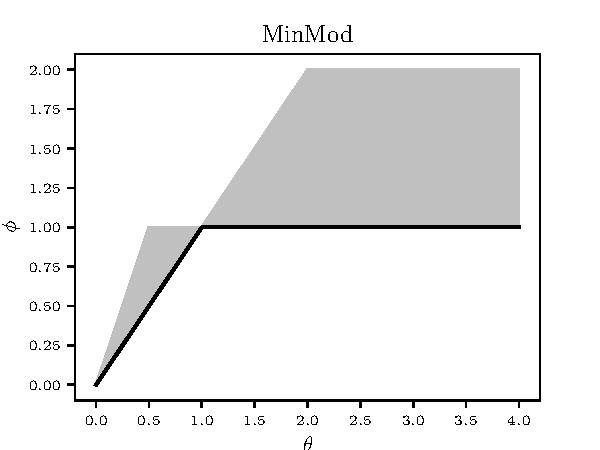
\includegraphics[width=0.24\textwidth]{figures/MinMod.pdf}
    \end{subfigure}
    \begin{subfigure}
    \centering
    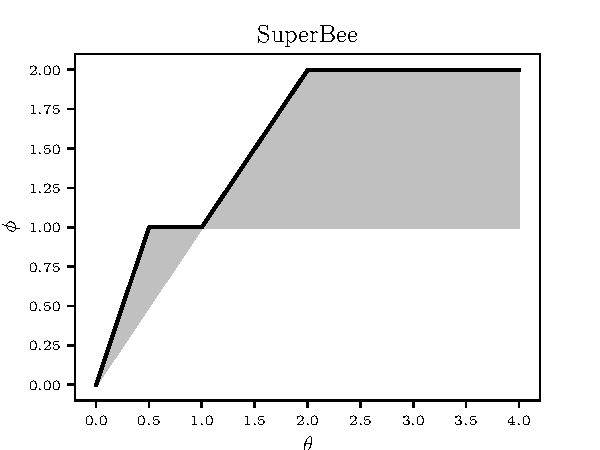
\includegraphics[width=0.24\textwidth]{figures/SuperBee.pdf}
    \end{subfigure}
    \begin{subfigure}
    \centering
    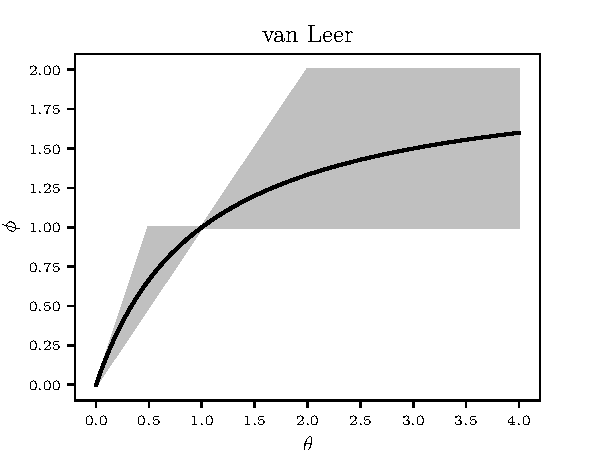
\includegraphics[width=0.24\textwidth]{figures/vanLeer.pdf}
    \end{subfigure}
    \begin{subfigure}
    \centering
    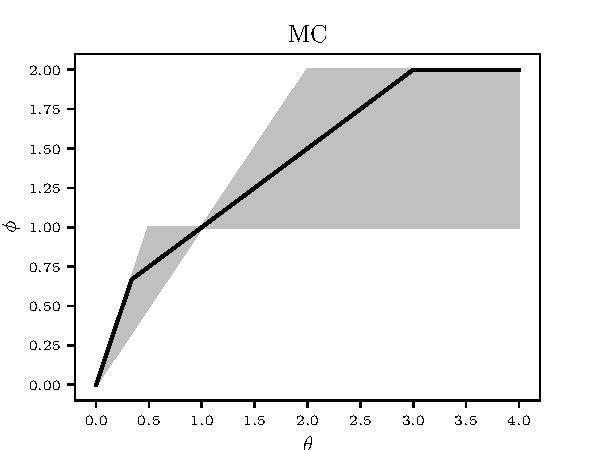
\includegraphics[width=0.24\textwidth]{figures/MC.pdf}
    \end{subfigure}
    \caption{The TVD region in $\phi-\theta$ space and the locations of the TVD limiters}
    \label{fig:tvd}
\end{figure}

\section{High Resolution in the Temporal Domain}
Until now, the developed methods were discrete in the both temporal and spatial domains. If we discretize a PDE in the temporal space first, it reduces the PDE to a system of ODEs, which can be solved using the known ODE solvers. This approach allows us to introduce higher order methods both in the spatial and the temporal domain, with decoupled issues of the discretizations of each domain. We can write the resulting semi-discrete version of the update formula as:
$$
    Q_i'(t) = -\frac{1}{\Delta x}[F_{i+1/2}(Q(t)) - F_{i-1/2}(Q(t))] = \mathcal{L}_i(Q(t))
$$
In this form, spatial and temporal discretizations are decoupled. For the spatial discretization, we can apply the previous knowledge about limiters and high-order methods. Then, we can apply more advanced methods for the time discretization. However, as in the spatial discretization, a special care must be taken while constructing the higher order methods in the temporal domain due to the possibility of the additional oscillations. In order to ensure that we do not add oscillations by our numerical methods, we again have to make sure that the method shows the TVD characteristic. TVD methods based on the semi discretization approach are easy to verify. If a spatial discretization method is a TVD method when the forward Euler time stepping is used, some of the high-order time stepping methods is guaranteed to be a TVD method too. These kind of time stepping methods are called strong stability-preserving (SSP) time discretizations. An example of one of these special methods is the two step Runge-Kutta time stepping:
$$
Q^*  = Q^n + \Delta t \mathcal{L}(Q^n)
$$
$$
Q^{**}  = Q^* + \Delta t \mathcal{L}(Q^*)
$$
$$
Q^{n+1}  = \frac{1}{2}(Q^n + Q^{**})
$$

\section{ENO Schemes}
For the high order reconstruction, we have chosen to switch from the piecewise constant polynomial to a piecewise linear polynomial. Naturally, one might think how to increase the degree of the polynomial even further. However, the problem is that we only have cell averages to construct the polynomial and if we try to increase the degree of the polynomial, number of free parameters would be much higher. Instead of approaching it blindly, consider a function such that:
$$
    w'(x) = q(x,t)
$$
and
$$ 
w(x) = \int_{x_{1/2}}^x q(\xi, t)d\xi
$$
where the lower bound of the integral is arbitrary. For example, a cell average can be used. Then we can write
$$
W_i = w(x_{i+1/2}) = \int_{x_{1/2}}^{x_{i + 1/2}} q(\xi, t)d\xi
$$
Then, given the cell averages, this function is going to yield the summation of the cell averages
$$
W_i = \Delta x \sum^i_{j=1} \Bar{q}_j (t)
$$
Basically, to approximate the $w$ in the cell $i$, we can use an interpolating polynomial of degree $s$, passing through $s+1$ points. 
\par
The flaw of this approach is that the cell averages should be smooth in those $s+1$ points. However, it is not the case for the most of the problems, especially the non-linear ones. Consider that we interpolate the values $W_{i-j},...,W_{i-j+s}$. High degree interpolant polynomials are highly oscillatory even for a smooth data. We can adapt the idea to minimize the oscillations, which was introduced in the limiter based methods, to this concept too. We need to choose the value j for each i such that the interpolating polynomials result in the smallest possible oscillations.
\par
To develop such a set of interpolant polynomials, one can use the Newton's divided difference method. Starting with the linear function of passing $W_{i-1}$ and $W_{i}$, one can write higher order functions recursively. Note that the divided differences of $W_i$ are directly related to the values $\Bar{q}_i$ too. Therefore, the values for $W_i$ are not calculated in practice. With this approach, one can obtain  arbitrary degree of polynomials depending on the smoothness of the region with high efficiency. This type of methods are called essentially non-oscillatory (ENO) methods. Another popular version of the vanillia ENO method is the weighted ENO (WENO) in which all the divided differences are used to calculate a weighted average. Since they are already calculated, this approach does not result in additional computational effort. Moreover, since this approach uses all the differences in the weighted manner, it has the capability to adapt itself in the smooth and discontinuous regions better than the vanilla version, which results in more robust method.

\section{Conclusion}
The higher-order methods for the conservation laws needs special attention due to their close relationship with the discontinuous solutions. Although the linear equations cannot result in discontinuous solutions with a smooth initial data, non-linear equations or linear equations with discontinuous initial data can. Therefore, the methods developed here mostly considered the discontinuous initial data on a linear conservation law, due to its simplicity and their representational power. These methods are easily extensible to non-linear equations too.
\par
The first approach, the Lax-Wendroff method, was to obtain a higher-order method using Taylor series expansion, which introduced non-physical oscillations to the solution. Then, it is improved using limiters to detect the smooth and discontinuous regions in the solution, and the corresponding TVD methods were discussed. Since we also want higher resolution in the temporal domain too, the semi-discrete approach was discussed. Finally, more advanced methods, which are based on the higher order polynomial reconstruction, ENO and WENO methods are developed. These are the main recipe for the higher-order methods and more advanced methods can be found on the literature with this background information.

% An example of a floating figure using the graphicx package.
% Note that \label must occur AFTER (or within) \caption.
% For figures, \caption should occur after the \includegraphics.
% Note that IEEEtran v1.7 and later has special internal code that
% is designed to preserve the operation of \label within \caption
% even when the captionsoff option is in effect. However, because
% of issues like this, it may be the safest practice to put all your
% \label just after \caption rather than within \caption{}.
%
% Reminder: the "draftcls" or "draftclsnofoot", not "draft", class
% option should be used if it is desired that the figures are to be
% displayed while in draft mode.
%
%\begin{figure}[!t]
%\centering
%\includegraphics[width=2.5in]{myfigure}
% where an .eps filename suffix will be assumed under latex, 
% and a .pdf suffix will be assumed for pdflatex; or what has been declared
% via \DeclareGraphicsExtensions.
%\caption{Simulation results for the network.}
%\label{fig_sim}
%\end{figure}

% Note that the IEEE typically puts floats only at the top, even when this
% results in a large percentage of a column being occupied by floats.


% An example of a double column floating figure using two subfigures.
% (The subfig.sty package must be loaded for this to work.)
% The subfigure \label commands are set within each subfloat command,
% and the \label for the overall figure must come after \caption.
% \hfil is used as a separator to get equal spacing.
% Watch out that the combined width of all the subfigures on a 
% line do not exceed the text width or a line break will occur.
%
%\begin{figure*}[!t]
%\centering
%\subfloat[Case I]{\includegraphics[width=2.5in]{box}%
%\label{fig_first_case}}
%\hfil
%\subfloat[Case II]{\includegraphics[width=2.5in]{box}%
%\label{fig_second_case}}
%\caption{Simulation results for the network.}
%\label{fig_sim}
%\end{figure*}
%
% Note that often IEEE papers with subfigures do not employ subfigure
% captions (using the optional argument to \subfloat[]), but instead will
% reference/describe all of them (a), (b), etc., within the main caption.
% Be aware that for subfig.sty to generate the (a), (b), etc., subfigure
% labels, the optional argument to \subfloat must be present. If a
% subcaption is not desired, just leave its contents blank,
% e.g., \subfloat[].


% An example of a floating table. Note that, for IEEE style tables, the
% \caption command should come BEFORE the table and, given that table
% captions serve much like titles, are usually capitalized except for words
% such as a, an, and, as, at, but, by, for, in, nor, of, on, or, the, to
% and up, which are usually not capitalized unless they are the first or
% last word of the caption. Table text will default to \footnotesize as
% the IEEE normally uses this smaller font for tables.
% The \label must come after \caption as always.
%
%\begin{table}[!t]
%% increase table row spacing, adjust to taste
%\renewcommand{\arraystretch}{1.3}
% if using array.sty, it might be a good idea to tweak the value of
% \extrarowheight as needed to properly center the text within the cells
%\caption{An Example of a Table}
%\label{table_example}
%\centering
%% Some packages, such as MDW tools, offer better commands for making tables
%% than the plain LaTeX2e tabular which is used here.
%\begin{tabular}{|c||c|}
%\hline
%One & Two\\
%\hline
%Three & Four\\
%\hline
%\end{tabular}
%\end{table}


% Note that the IEEE does not put floats in the very first column
% - or typically anywhere on the first page for that matter. Also,
% in-text middle ("here") positioning is typically not used, but it
% is allowed and encouraged for Computer Society conferences (but
% not Computer Society journals). Most IEEE journals/conferences use
% top floats exclusively. 
% Note that, LaTeX2e, unlike IEEE journals/conferences, places
% footnotes above bottom floats. This can be corrected via the
% \fnbelowfloat command of the stfloats package.


% if have a single appendix:
%\appendix[Proof of the Zonklar Equations]
% or
%\appendix  % for no appendix heading
% do not use \section anymore after \appendix, only \section*
% is possibly needed

% use appendices with more than one appendix
% then use \section to start each appendix
% you must declare a \section before using any
% \subsection or using \label (\appendices by itself
% starts a section numbered zero.)
%

% Can use something like this to put references on a page
% by themselves when using endfloat and the captionsoff option.
\ifCLASSOPTIONcaptionsoff
  \newpage
\fi



% trigger a \newpage just before the given reference
% number - used to balance the columns on the last page
% adjust value as needed - may need to be readjusted if
% the document is modified later
%\IEEEtriggeratref{8}
% The "triggered" command can be changed if desired:
%\IEEEtriggercmd{\enlargethispage{-5in}}

% references section

% can use a bibliography generated by BibTeX as a .bbl file
% BibTeX documentation can be easily obtained at:
% http://mirror.ctan.org/biblio/bibtex/contrib/doc/
% The IEEEtran BibTeX style support page is at:
% http://www.michaelshell.org/tex/ieeetran/bibtex/
%\bibliographystyle{IEEEtran}
% argument is your BibTeX string definitions and bibliography database(s)
%\bibliography{IEEEabrv,../bib/paper}
%
% <OR> manually copy in the resultant .bbl file
% set second argument of \begin to the number of references
% (used to reserve space for the reference number labels box)
\appendices
\section{Implementations of the Methods}
A simple Python code to solve linear advection equation and Burger's equation (experimental) with several limiters can be found in \href{http://github.com/oguzziya/high-order-fv}{\textit{github.com/oguzziya/high-order-fv}}.

\begin{thebibliography}{1}

\bibitem{IEEEhowto:leveq}
R.J.~Leveque, \emph{Finite-Volume Methods for Hyperbolic Problems}, 2nd~ed.\hskip 1em plus
  0.5em minus 0.4em\relax Cambridge, England: Cambridge University Press, 2004.

\bibitem{IEEEhowto:toro}
E.F.~Toro, \emph{Riemann Solvers and Numerical Methods for Fluid Dynamic, A Practical Introduction}, 3rd~ed.\hskip 1em plus
  0.5em minus 0.4em\relax Heidelberg, Germany: Springer, 2009.

\bibitem{IEEEhowto:highorder}
T.J.~Barth and H.~Deconinck, \emph{High-Order Methods for Computational Physics}, 1st~ed.\hskip 1em plus
  0.5em minus 0.4em\relax Heidelberg, Germany: Springer, 1999.

\end{thebibliography}



% biography section
% 
% If you have an EPS/PDF photo (graphicx package needed) extra braces are
% needed around the contents of the optional argument to biography to prevent
% the LaTeX parser from getting confused when it sees the complicated
% \includegraphics command within an optional argument. (You could create
% your own custom macro containing the \includegraphics command to make things
% simpler here.)
%\begin{IEEEbiography}[{\includegraphics[width=1in,height=1.25in,clip,keepaspectratio]{mshell}}]{Michael Shell}
% or if you just want to reserve a space for a photo:

% if you will not have a photo at all:
% insert where needed to balance the two columns on the last page with
% biographies
%\newpage

% You can push biographies down or up by placing
% a \vfill before or after them. The appropriate
% use of \vfill depends on what kind of text is
% on the last page and whether or not the columns
% are being equalized.

%\vfill

% Can be used to pull up biographies so that the bottom of the last one
% is flush with the other column.
%\enlargethispage{-5in}



% that's all folks
\end{document}